\section{Aufbau}
\label{sec:Aufbau}

Der an eine Hochspannung angeschlossene Detektor befindet sich zur Abschirmung der kosmischen Strahlung in einem Bleikasten, der im Inneren mit einer Kupferschicht ausgekleidet ist, um eventuelle $\beta$-Strahlung durch Blei-Isotope abzuschirmen. 
Um die durch Sammlung der Ladungsträger entstehenden Signale möglichst verlustfrei weiterzuleiten, wird über einen Operationsverstärker, der über eine Kapazität $C_.K$ rückgekoppelt wird, der Strom der ankommenden Elektronen in eine Spannung umgewandelt. 
Damit einzelne Impulse gemessen werden können, muss der Kondensator nach jedem Impuls entladen werden. Um das Verstärkerrauschen zu minimieren, wird dazu kein Widerstand verwendet, sondern die Gate-Drain-Schicht des Feldeffekttransistors nach jedem Puls mit einer über einen Schwellendiskriminator mit dem Verstärker verbundenen LED bestrahlt, wodurch er leitend wird und die Ladung abfließen kann. Das Schaltbild dieses Vorverstärkers ist in Abbildung \ref{fig:Schalt} zu sehen.
Über ein RC-Glied wird dieser an den Hauptverstärker gekoppelt, der die Spannungen über Hoch- und Tiefpässe glättet und auf $0$ - $\SI{10}{\volt}$ verstärkt, da der angeschlossene Analog-Digital-Konverter(ADC) nur für diesen Bereich ausgelegt ist. Um zu verhindern, dass bei schnell hintereinander eintreffenden Pulsen ein verfälschtes Signal aufgenommen wird, wird der Eingang des Konverters nach Ankommen des Spannungspulses über eine Steuereinheit gesperrt. Dadurch kommt es allerdings zu einer Totzeit in der keine Impulse detektiert werden können, sodass nicht die gesamte Aktivität einer Probe bestimmt werden kann.
Der ADC selbst besteht aus einem Kondensator und einer Konstantstromquelle, die ihn mit einem gleichmäßigen Strom entlädt.
Solange dieser Strom fließt, ist ein UND-Gatter geöffnet, durch das regelmäßige Pulse eines Quarz-Oszillators geschickt und von einem Binärzähler gezählt werden.
Je länger das Gatter geöffnet ist, desto mehr Pulse kommen hindurch, sodass ihre Anzahl ein Maß für die im Detektor deponierte Energie ist und der Inhalt der entsprechenden Kanalnummer am Rechner um 1 erhöht wird. Der Aufbau des ADC ist in Abbildung \ref{fig:Schalt2} zu sehen. 
Um zu verhindern, dass der Detektor im ungekühlten Zustand an die Hochspannung angeschlossen wird, ist an seinem Gehäuse ein Temperaturfühler angebracht, der in diesem Fall die Hochspannung blockiert. Ein Block-Schaltbild des gesamten Aufbaus ist in Abbildung \ref{fig:Schalt3} zu sehen, wobei der Vielkanalanalysator den ADC und den Binärzähler bezeichnet, der an den Rechner angeschlossen ist.

\begin{figure}
	\centering
	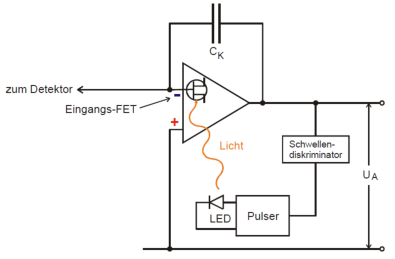
\includegraphics[width=\linewidth-70pt,height=\textheight-70pt,keepaspectratio]{content/images/Schaltung.pdf}
	\caption{Schematischer Aufbau der Vorverstärkerschaltung\cite{V18}.}
	\label{fig:Schalt}
\end{figure}
\begin{figure}
	\centering
	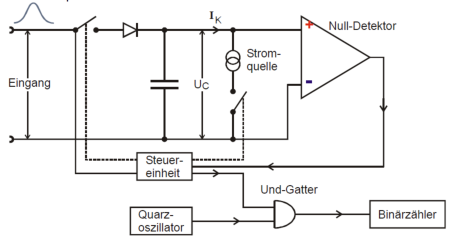
\includegraphics[width=\linewidth-70pt,height=\textheight-70pt,keepaspectratio]{content/images/Schaltung2.pdf}
	\caption{Schematischer Aufbau des Hauptverstärkers\cite{V18}.}
	\label{fig:Schalt2}
\end{figure}
\begin{figure}
	\centering
	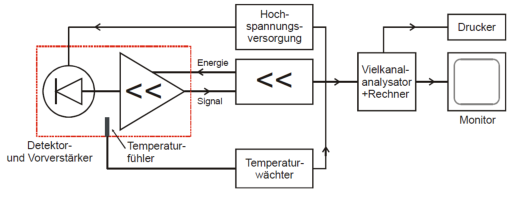
\includegraphics[width=\linewidth-70pt,height=\textheight-70pt,keepaspectratio]{content/images/Schaltung3.pdf}
	\caption{Schematischer Aufbau der gesamten Schaltung\cite{V18}.}
	\label{fig:Schalt3}
\end{figure}
